\section{Cross Section}
We are only interested in the interactions $Q_{2bs}$, respectively $Q_{2sb}$, therefore all coefficients $C_{lij}$ vanish except $C_{2sb} = C_{2bs}^*$. In terms of the coefficients in \eqref{eq:CoeffNormal} this means
\begin{align}
	K_{1,d} &= +\text{Re}(V_{cd}^*V_{td}C_{2sb})\notag \\
	K_{1,s} &= +\text{Re}(V_{cs}^*V_{ts}C_{2sb})\notag \\
	K_{3,d} &= -\text{Re}(V_{cd}^*V_{td}C_{2sb})\notag \\
	K_{3,s} &= -\text{Re}(V_{cs}^*V_{ts}C_{2sb}) \ ,
\end{align}
and all other $K_{l,q}=0$. These are the coefficients of the spin-dependent interaction $R_{3,q} = (\bar{\chi}\gamma^\mu\chi)(\bar{q}\gamma_\mu\gamma_5 q)$ and the spin-independent interaction $R_{1,q} = (\bar{\chi}\gamma^\mu\chi)(\bar{q}\gamma_\mu q)$. We neglect the former one because the spin-dependant cross section is various orders of magnitude smaller than the spin-independent cross section. Since nucleons consist of up and down quarks, we abolish the interaction with strange quarks as they are only available as sea quarks. We are left with the spin-independent vector interaction
\begin{align}
	\mathcal{L} = K_{1,d}(\bar{\chi}\gamma^\mu\chi)(\bar{d}\gamma_\mu d) \ .
\end{align}
As is explained in \cite[Chapter 7]{Supersymmetric}, this operator basically counts the number of down quarks in the nucleus, so the nucleon cross section is
\begin{align}
	\sigma_{0,\text{tree}}^\text{SI} &= \frac{\mu_{A\chi}^2}{A^2\pi}\left|ZC_p +(A-Z)C_n\right|^2 \ ,
\end{align}
where $C_p = K_{1,d}$ is the proton coefficient and $C_n = 2K_{1,d}$ is the neutron coefficient.


Interestingly, $C_{2bs}$ does not depend on $g'$ or $m_{Z'}$, but reads $C_{2bs} = q_\chi\frac{Y_{Qb}Y_{Qs}^*}{2m_Q^2}$, for which \cite{InColour} gives the approximation
\begin{align}\label{eq:BoundC}
	\text{Re}\left(C_{2bs}\right) \approx \SI{8e-10}{\giga\electronvolt}^{-2} \ .
\end{align}
\begin{figure}
	\centering
	\begin{tikzpicture}
\tikzstyle{centerArrow}=[decoration={
markings,
mark=at position 0.5 with {\fill (2pt,0)--(-2pt,2.31pt)--(-2pt,-2.31pt)--cycle;}}]
\begin{scope}[xshift=3cm,yshift=-2cm]
\def\xmove{2}
\def\ymove{1.25}
\def\centerShift{2}
\def\centerSize{0.08cm}
\coordinate (tCenter1) at (0,0);
\coordinate[fill, circle,inner sep=\centerSize] (tCenter2) at (0,-\centerShift cm);
\node (upperLeft) at (-\xmove,\ymove) {$\chi$};
\node (upperRight) at (\xmove,\ymove) {$\chi$};
\node (lowerLeft) at (-\xmove,-\centerShift cm-\ymove cm) {$b_L,s_L$};
\node (lowerRight) at (\xmove,-\centerShift cm-\ymove cm) {$s_L,b_L$};
\node at (0.5,-\centerShift/2) {$Z'$};
\draw [centerArrow,postaction={decorate}]  (upperLeft) -- (tCenter1) ;
\draw [centerArrow,postaction={decorate}]  (tCenter1) -- (upperRight) ;
\draw [centerArrow,postaction={decorate}]  (lowerLeft) -- (tCenter2) ;
\draw [centerArrow,postaction={decorate}]  (tCenter2) -- (lowerRight) ;
\draw [decoration={snake, segment length=1.5mm, amplitude=0.5mm},decorate] (tCenter1) -- (tCenter2) ;
\end{scope}
\end{tikzpicture}
	\caption{Tree level diagram for direct detection considering flavour mixing.}
	\label{fig:DD}
\end{figure}
\todo{Wieso ist eigentlich $Q_L^2\gamma_\mu Q_L^3 = s_L\gamma_\mu b_L$?}

\section{Results}
We now compare the nucleon cross sections for the loop interaction $\sigma_{0,\text{Loop}}$ (see figure \ref{fig:Loop}) and the tree level interaction $\sigma_{0,\text{tree}}$ (see figure \ref{fig:DD}) considering flavour mixing.

We first consider the choice $q_l\approx q_\chi= 1$. The dark matter mass cannot be much larger than $\SI{23}{\giga\electronvolt}$ in this case \cite{Z}. For the allowed $m_\chi$ region, figure \ref{fig:Allgemein11} shows the loop cross section in the bounds \eqref{eq:BoundBS} as shaded red area. For $C_{2bs}$ we tried various viable values that are in accordance with \eqref{eq:BoundC}, setting $\text{Im}(C_{2bs})$ to the same magnitude as $\text{Re}(C_{2bs})$.
\begin{figure}
	\centering
	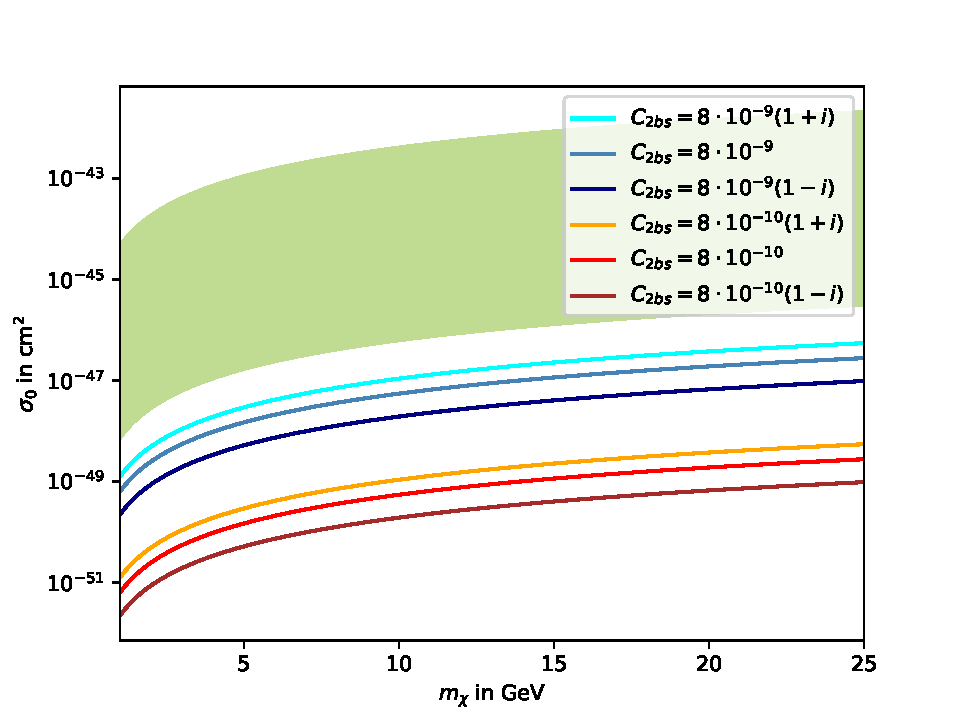
\includegraphics[scale=.8]{content/graphics/Allgemein11.pdf}
	\caption{Comparison of nucleon cross sections for $q_l=q_\chi=1$. The shaded red area represents $\sigma_{0,\text{Loop}}$ with the bounds in \eqref{eq:BoundBS}. The coloured lines show $\sigma_{0,\text{tree}}$ for different values of $C = C_{2bs}$ (in $\si{\giga\electronvolt}^{-2}$).}
	\label{fig:Allgemein11}
\end{figure}



Since there is no restriction to $\text{Im}(C_{2bs})$, we can as well set it to higher values. As shown in figure \ref{fig:HighIm11} this obviously leads to larger $\sigma_{0,\text{tree}}$, reaching the order of magnitude of $\sigma_{0,\text{Loop}}$.
\begin{figure}
	\centering
	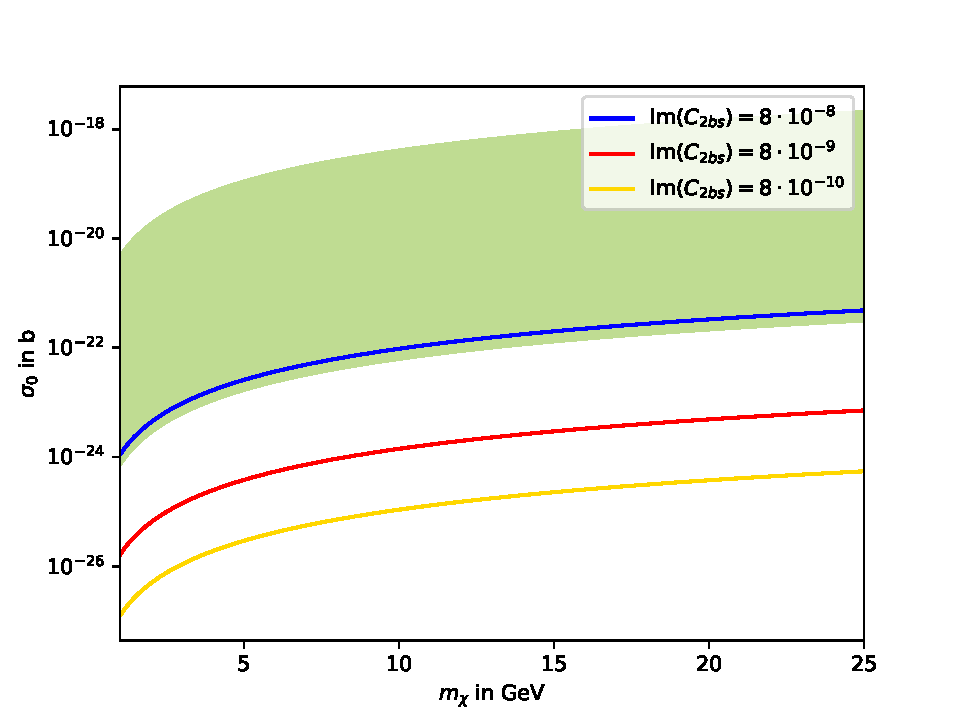
\includegraphics[scale=.8]{content/graphics/Im11.pdf}
	\caption{Comparison of nucleon cross sections for $q_l=q_\chi=1$. The shaded red area represents $\sigma_{0,\text{Loop}}$ with the bounds in \eqref{eq:BoundBS}. The coloured lines show $\sigma_{0,\text{tree}}$ for different choices of $\text{C} = \text{Im}(C_{2bs})$. The real part of $C_{2bs}$ is fixed at $\SI{8e-10}{\giga\electronvolt}^{-2}$.}
	\label{fig:HighIm11}
\end{figure}




Second we follow \cite{Z} and examine the case $q_l=1,q_\chi=\sfrac{1}{6}$. Here we have no restrictions for $m_\chi$. In figure \ref{fig:Allgemein116} we present the loop cross section in the bounds \eqref{eq:BoundBS} again as shaded red area and tried values for $C_{2bs}$ accordingly to above. Due to $\sigma_0\propto q_\chi^2$, there is no qualitative change as to figure \ref{fig:Allgemein11}.
\begin{figure}
	\centering
	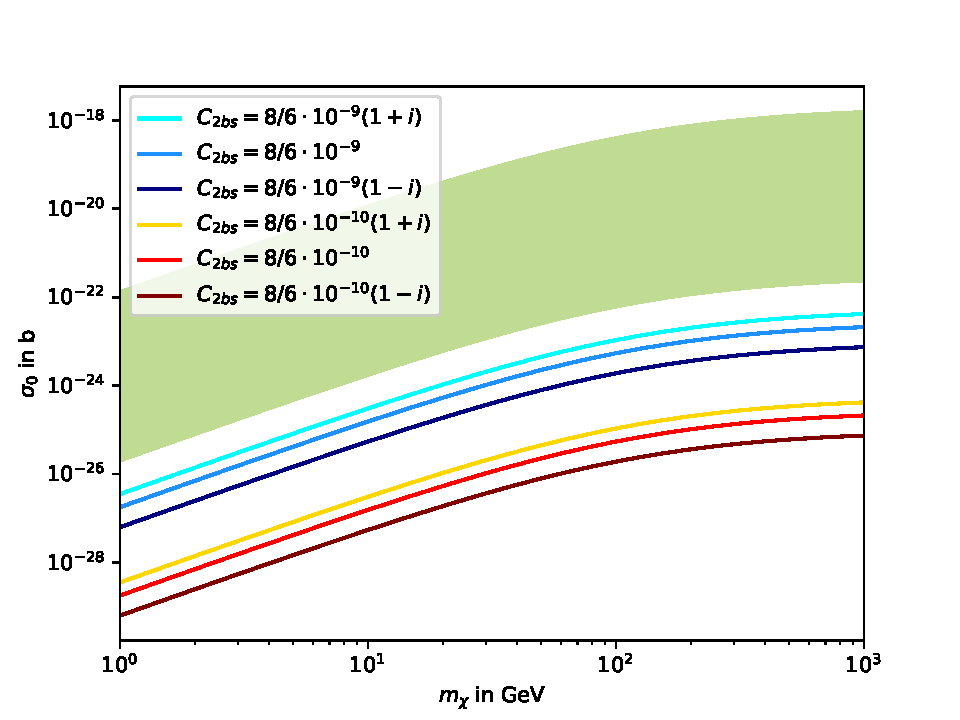
\includegraphics[scale=.8]{content/graphics/Allgemein116.pdf}
	\caption{Comparison of nucleon cross sections for $q_l=1,q_\chi=\sfrac{1}{6}$. The shaded red area represents $\sigma_{0,\text{Loop}}$ with the bounds in \eqref{eq:BoundBS}. The coloured lines show $\sigma_{0,\text{tree}}$ for different values of $C = C_{2bs}$ (in $\si{\giga\electronvolt}^{-2}$).}
	\label{fig:Allgemein116}
\end{figure}



Enlarging $\text{Im}(C_{2bs})$ gives the same results as above.
\begin{figure}
	\centering
	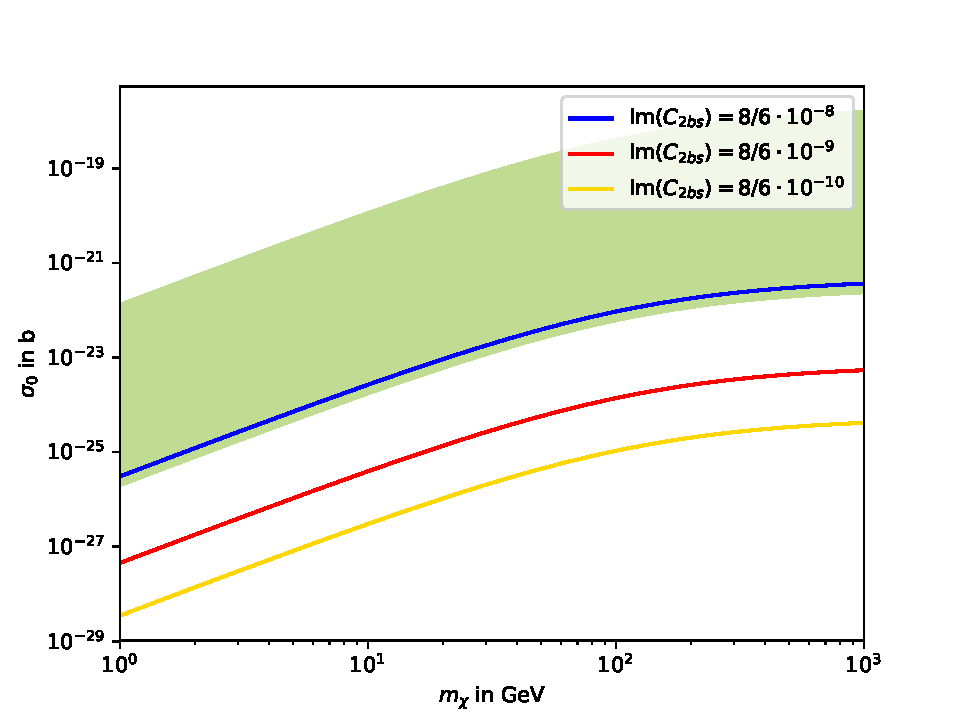
\includegraphics[scale=.8]{content/graphics/Im116.pdf}
	\caption{Comparison of nucleon cross sections for $q_l=q_\chi=1$. The shaded red area represents $\sigma_{0,\text{Loop}}$ with the bounds in \eqref{eq:BoundBS}. The coloured lines show $\sigma_{0,\text{tree}}$ for different choices of $\text{C} = \text{Im}(C_{2bs})$. The real part of $C_{2bs}$ is fixed at $\SI{8e-10}{\giga\electronvolt}^{-2}$.}
	\label{fig:HighIm116}
\end{figure}